\section{Simulation Analysis and the Path for the Greater Good}

For this analysis, we used the BC557A model for the PNP-transistor and the BC547A model for the NPN-transistor, from Philips available in \textit{Ngspice}, having then created the circuit presented in Fig. \ref{fig:bigscheme} (it was using Ngspice that we determined, in fact, what was the best circuit for our purposes). \\

The use of a bypass capacitor, $C_B$, in parallel with a resistor on the gain stage has the main objective of "absorbing" AC noise in order to produce a cleaner DC signal. On the other hand, the output coupling capacitor used, $C_o$, is used to filter the signal, passing the wanted AC signal and blocking the undesired DC components. Finally, we also used a input coupling capacitor, which value should be sufficiently high to allow us to obtain a small value for the lower cutoff frequency.\\

Besides this there was not a lot more information to conclude what was the maximum of the function merit like a closed formula so our approach was based on incremental modification in order to understand the purpose of each component in the circuit each is was summarized in the effect on the gain (g), bandwidth (BW) and lower cutoff frequency (lCf).\\

It was concluded that the increase in $C_O$  would decreses the lCf; the increase in $R_{out}$ increses g and decreases BW; the increase in $C_B$ decreases lCf; $R_E$ and $R_C$ increases seem to have a similar effect, decreasing BW, a by a lot less g and lCf; $R_1$ and $R_2$ seem to be very unstable needing to be at very special values to mantain the transistor in the active zone and at last $C_i$, increase causes a decrease in lCf. Then it was a matter of maximizing the merit function understanding what is being increased and decreased.\\

Finally, one found the values considered as the best to find an optimal merit score which are given by:

\begin{table}[H]
    \centering
    \begin{tabular}{|c|c|c|||c|c|c|}
    \hline
        \textbf{Component} & \textbf{Value} & \textbf{Cost} & \textbf{Component} & \textbf{Value} & \textbf{Cost} \\
        \hline
        \hline
        $R_{in}$ & $100\Omega$ & $0.1$ & $C_i$ & $135\mu$F & 135\\
        \hline
        $R_{1}$ & $90k\Omega$ & $90$ & $T_{NPN}$ & - & 0.1\\
        \hline
        $R_{2}$ & $10k\Omega$ & $10$ & $T_{NPN}$ & - & 0.1\\
        \hline
        $R_{E}$ & $120\Omega$ & $0.12$ & $C_B$ & $1840\mu$F & 1840\\
        \hline
        $R_{C}$ & $2.3k\Omega$ & $2.3$ & $R_{out}$ & $330\Omega$ & 0.33\\
        \hline
        $R_{L}$ & $8\Omega$ & $0.008$ & $C_o$ & $1200\mu$F & 1200\\
        \hline
    \end{tabular}
    \caption{Values of the components used on Fig. \ref{fig:bigscheme}.}
    \label{tab:tentativas}
\end{table}


\subsection{Cost and Merit Score}
Evaluating the merit, and knowing that the cost is given by \eqref{eq:cost}
\begin{equation}
    cost = 2 \cdot 0.1 + (0.1+90+10+0.12+2.3+0.008+0.33) + (135+1840+1200) =  3278.06\text{MU}
    \label{eq:cost}
\end{equation}

%Using the values obtained for $c$, $d$ and $r$, one can finally calculate the merit score obtained with this circuit (calculated using equation \eqref{score}), which allows one to get the following score:

%\begin{equation}
    %M = 3.31752e+02
%\end{equation}

\subsection{Gain stage}
To understand the role played by the gain stage this circuit one plotted the results obtained for the gain and phase at the end of this stage which is between node 5 and ground.

\vspace{-70px}
\begin{figure}[H]
    \centering
    \vspace{-50px}
    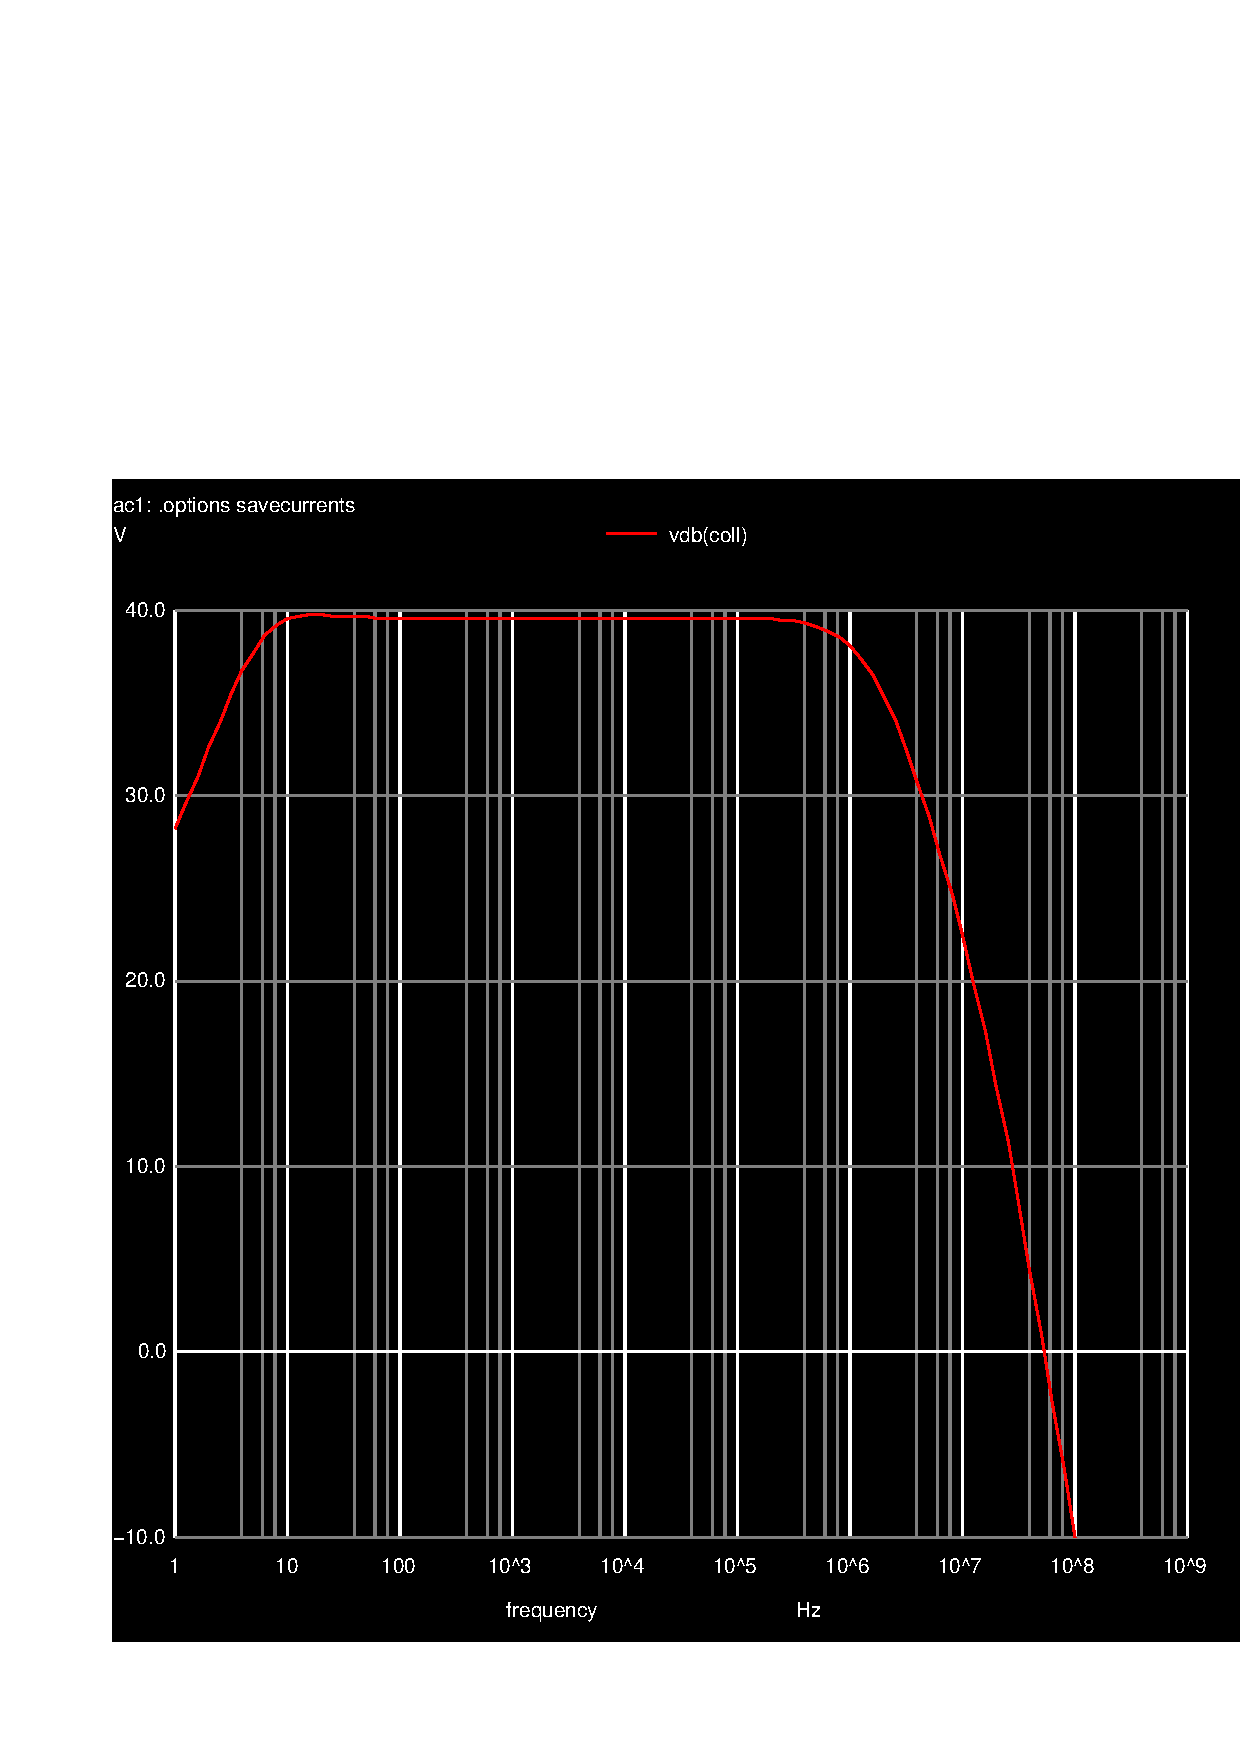
\includegraphics[width = 0.7\textwidth]{sim/gainplotdb.pdf}
    \vspace{-30px}
    \caption{\textit{Plot} obtained at the end of the gain stage}
    \label{fig:gaindb}
\end{figure}

\subsection{Output stage}
In this stage the output signal will be analysed, which is the voltage difference in the resistor $R_L$, but the main goal of this stage is to minimize the output impedance.

\vspace{-70px}
\begin{figure}[H]
    \centering
    \vspace{-50px}
    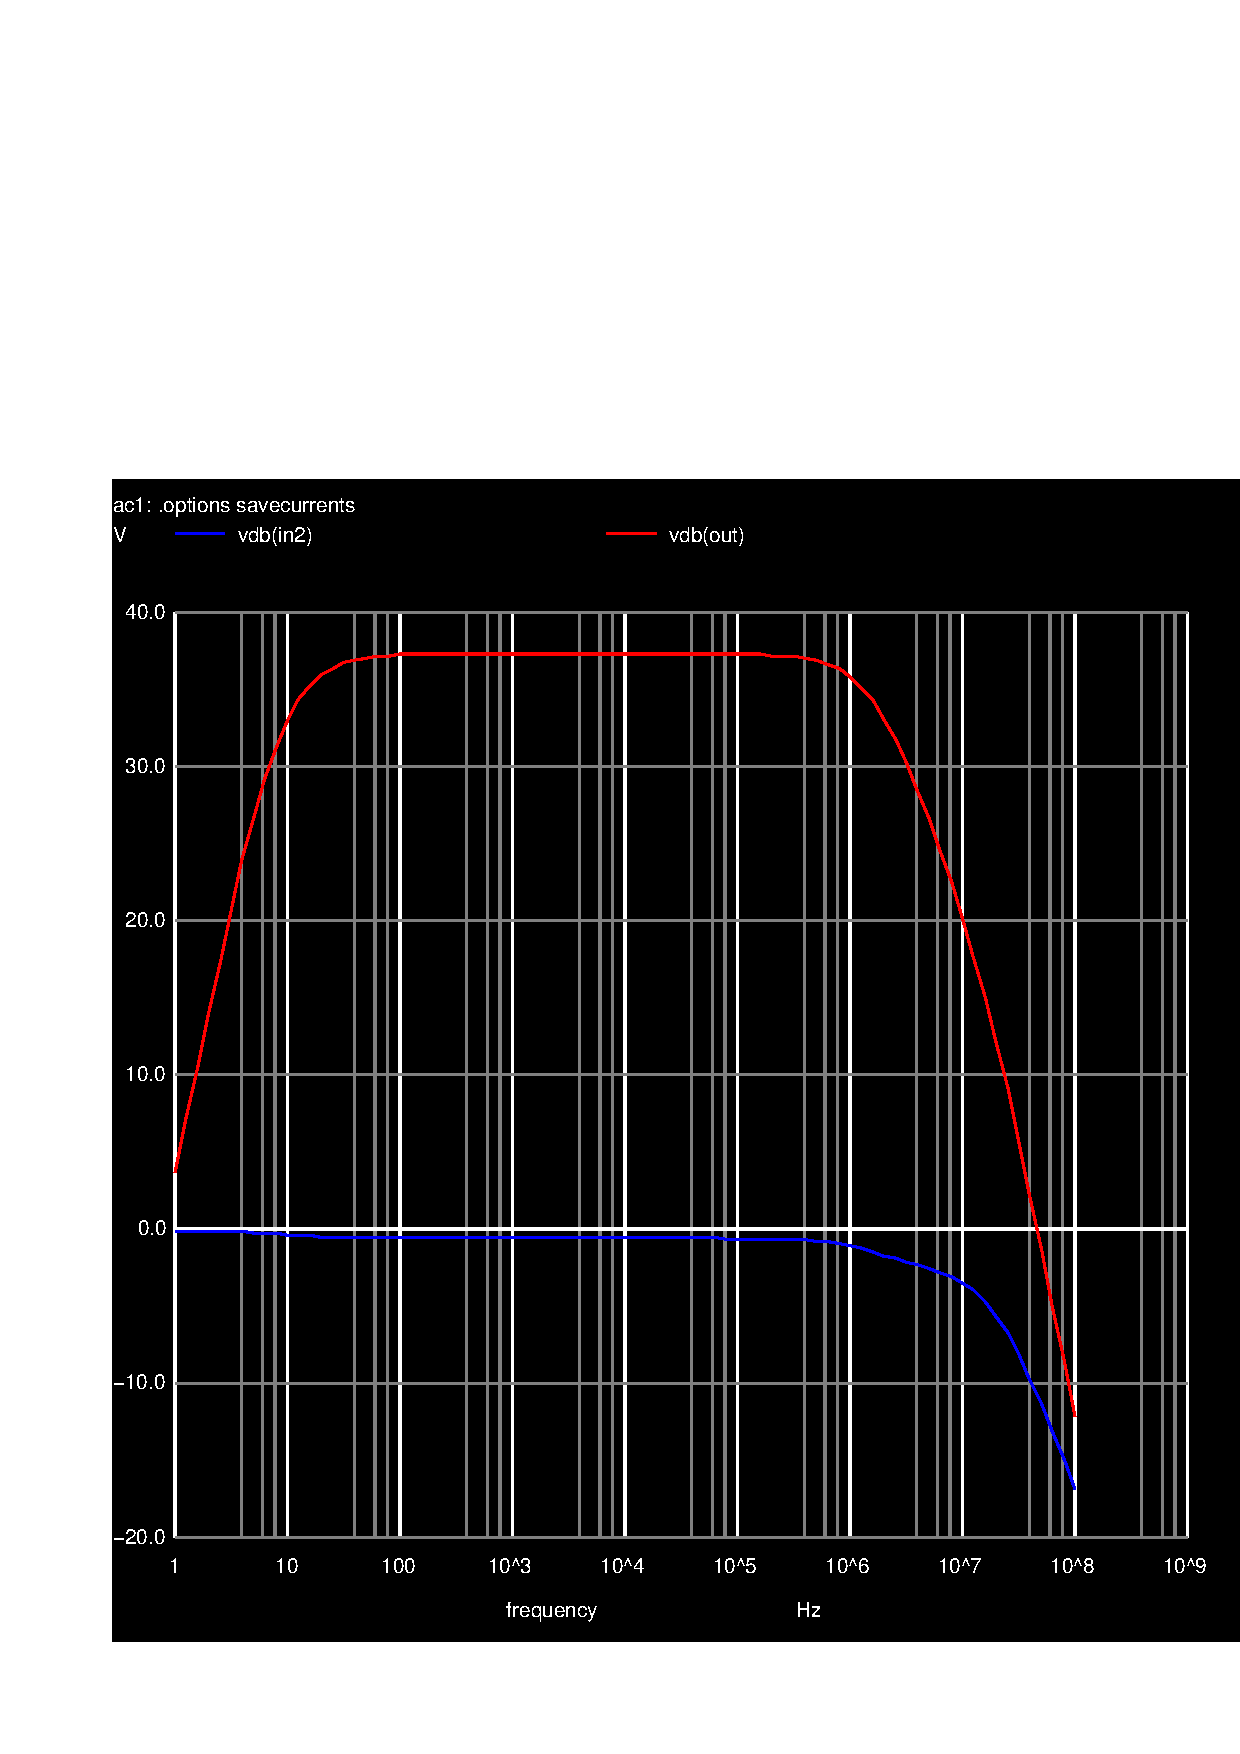
\includegraphics[width = 0.7\textwidth]{sim/vdbout.pdf}
    \vspace{-30px}
    \caption{\textit{Plot} obtained for the dB voltage at the circuit output and comparison with the initial dB voltage at the circuit input}
    \label{fig:output}
\end{figure}

\subsection{Values obtained and impedances}
Resuming, in the following table, we present the values obtained in \textit{Ngspice} for some relevant quantities as the gain, the lower and higher cut-off frequencies, the bandwidth ort the final merit score obtained:

\begin{table}[H]
    \centering
    \begin{tabular}{c|c}
        \textbf{Quantity} & \textbf{Value}\\
        \hline
        \hline
        Gain & 73.2378 V\\ \hline
Gain (dB) & 37.2947 dB\\ \hline
Lower cut-off frequency & 12.5855 Hz\\ \hline
Upper cut-off frequency & 1.57176E+06 Hz\\ \hline
Bandwidth & 1.57175E+06 Hz\\ \hline
Cost & 3278.06 MU\\ \hline
Merit & 2790.17\\ \hline

    \end{tabular}
    \caption{Relevant quantities obtained on \textit{Ngspice} simulation}
    \label{tab:quantities}
\end{table}

As anticipated on the introduction, one should have a high input impedance and a small output impedance. The values obtained through the \textit{Ngspice} simulation were for the input impedance were:

\begin{table}[H]
    \centering
    \begin{tabular}{c|c}
        \textbf{Quantity} & \textbf{Value}\\
        \hline
        \hline
        Zi & 1385.89 + (-36.7344)j $\Omega$\\ \hline
|Zi| & 1386.38 $\Omega$\\ \hline

    \end{tabular}
    \caption{Values obtained for the input impedance}
    \label{tab:zin}
\end{table}

And for the output impedance were:

\begin{table}[H]
    \centering
    \begin{tabular}{c|c}
        \textbf{Quantity} & \textbf{Value}\\
        \hline
        \hline
        Zo & 14.0507 + (0.625162)j $\Omega$\\ \hline
|Zo| & 14.0646 $\Omega$\\ \hline

    \end{tabular}
    \caption{Values obtained for the output impedance}
    \label{tab:zout}
\end{table}